\documentclass{article}

% Language setting
% Replace `english' with e.g. `spanish' to change the document language
\usepackage[english]{babel}

% Set page size and margins
% Replace `letterpaper' with `a4paper' for UK/EU standard size
\usepackage[letterpaper,top=1cm,bottom=1cm,left=2cm,right=2cm,marginparwidth=1.75cm]{geometry}

% Useful packages
\usepackage{amsmath}
\usepackage{graphicx}
\usepackage[colorlinks=true, allcolors=blue]{hyperref}


\usepackage{geometry}
\usepackage{booktabs}
\usepackage{longtable}
\usepackage{float}




\title{Social-Media-as-Predictive-Information-for-Stock-Market}
\author{Aristide Mawuena, Matthieu Baucher, Luca Hachani}

\begin{document}
\maketitle

\begin{abstract}
Financial social media like StockTwits holds rich discussion on public companies, with users sharing opinions, news reactions, and optional Bullish/Bearish labels. This text enables two key research questions: Can NLP models accurately infer an investor's market stance from their post? And does this sentiment predict future stock performance?
\end{abstract}

\section*{Introduction}

...

\section{Training Sentiment Labelling}
\subsection{Data preparation and selection}
For the study, we took all the messages and kept those annotated, I balanced the number of BULLISH/BEARISH for training and testing.
The messages were modified to remove any mention of their ticker in order not to learn the popularity of the symbols but rather the meaning of the sentences.
The tickers considered are TSLA, AAPL, AMD, NVDA, GOOGL, META : chosen because users who talk about one will talk about the others and that helps to generalize when creating a user embedding to add context for the prediction.


\begin{longtable}{lccccc}
\caption{Performance of models} \\
\toprule
   {\small mpnet-base} 
 & {\small electra-base-discriminator} 
 & {\small twitter-roberta-base-sentiment} 
 & {\small twitter-roberta-base} 
 & {\small finbert-tone} \\
\midrule
81.7\% & 82.4\% & 82.9\% & 82.9\% & 82.0\% \\
\bottomrule
\end{longtable}
\vspace{1mm}
distilroberta-base, albert-large-v2, electra-small-discriminator where tested and eliminated quickly. 
twitter-roberta-base-sentiment is quickly good and becomes the best with heavy 
training. The model is medium-sized. We therefore chose it to continue the study.
But Some tweets are more easily categorizable: notably longer tweets.

\begin{table}[H]
\caption{Accuracy on balanced dataset depending on the number of tokens in the message}
\centering
\begin{tabular}{cccc}
\toprule
T$\le$32 & 32$<$T$\le$64 & 64$<$T$\le$128 & 128$<$T$\le$256 \\
\midrule
82.5\% & 88.0\% & 91.9\% & 91.1\% \\
\bottomrule
\end{tabular}

\vspace{2mm}
{\centering \small Training on 1500000 messages and testing on 15000 tweets.\par}

\end{table}
\vspace{3mm}
For the study, we used a bounded token list to allow a huge gpu performance gain and lower memory usage : first tweets under 32 then between 32 and 64 (less numerous) etc.
To interpret a generated embedding, the best was to retrieve a layer of the model rather (and add a simple layer) than making a fully connected network.
One must especially not train the transformer for more than two epochs otherwise it learns by heart: we see the loss decrease but the performance does not increase (or even decreases). The solution is to use many messages (which is quite slow to process).

\subsection{Adding context to improve prediction}

We used 1500000 messages for training (for RAM reasons)

2 ideas:
\begin{itemize}

    \item Some users have their own way of expressing themselves and it is interesting to give a description of the user: we can represent it as the average of their previous embeddings (all tickers combined). The embedding thus obtained is reduced to a latent of dimension 2 for generalization.
    
    \item Some messages are neutral and come in response to others; some are ambiguous: A first idea consists in taking into account the previous messages to see if we can clarify these tweets: each tweet produces an embedding and we create a previous column which is a weighted average of the previous tweet with a basic attention mechanism:
    \texttt{current\_mean := (previous\_embedding + current\_mean) / 2}\\
    the embedding thus obtained is also reduced to a latent of dimension 2 for generalization.

\end{itemize}

\begin{figure}[h]
\centering
\noindent\makebox[\textwidth][c]{%
    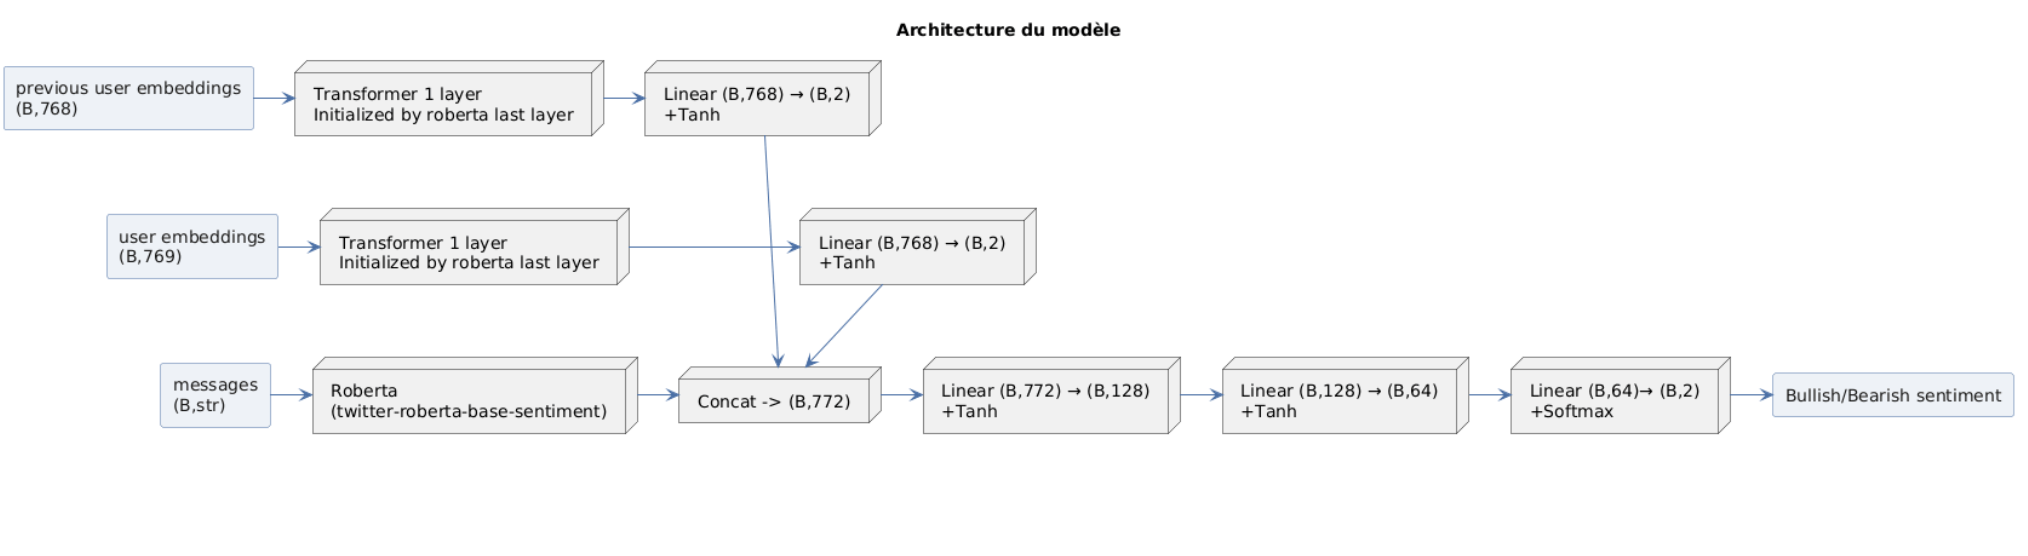
\includegraphics[width=1.2\textwidth]{schéma.png}
}
\caption{General diagram of the model with previous embedding and user embedding}
\end{figure}


\begin{center}
\textbf{Performances evaluated on 60000 tweets}
\end{center}

\begin{center}
\begin{tabular}{lc}
\toprule
Model used & performances \\
\midrule
roberta + simple classification head & 83.14\% \\
adding user embedding & 88.24\% \\
adding previous embedding & 86.19\% \\
adding previous embedding and user embedding & 88.72\% \\
\bottomrule
\end{tabular}
\end{center}

\begin{center}
\textbf{Performances evaluated on 15000 tweets, by number of tokens}
\begin{tabular}{lcccc}
\toprule
 & T$\le$32 & 32$<$T$\le$64 & 64$<$T$\le$128 & 128$<$T$\le$256 \\
\midrule
roberta + simple classification head & 82.5\% & 88.0\% & 91.9\% & 91.1\% \\
adding user embedding & 88.9\% & 91.4\% & 89.4\% & 91.1\% \\
adding previous embedding & 86.6\% & 86.7\% & 88.6\% & 90.2\% \\
adding previous embedding and user embedding & 89.1\% & 89.6\% & 88.7\% & 90.3\% \\
\bottomrule
\end{tabular}
\end{center}

Context give a significant gain for short messages (<64 for user embedding, <32 for previous embedding). On long tweets (which are much less numerous), we note a slight drop in performance. But the overall performance improves. If we took the max performances for each model, we see that we would reach 90\% overall ...

\subsection{Conclusion for labelling sentiment}
We can therefore have a very good prediction of tweets by taking into account the personality of the user and their previous tweets, even with ambiguous tweets.
Adding context is a good idea to improve overall performances ...

\subsection{Remaining points}

\begin{itemize}
\item  It would be interesting to provide the number of tokens to the model so that it can learn to trust more the user embedding when it has enough tokens (and therefore use less the context information) : With a little more time on this project, this would have been the next step.
\item  We could try to improve the handling of previous messages: tune the attention better
\item  Handle tweets that are replies, add the initial tweet in context
\item  It would be interesting to see if a user embedding remains credible for a long time if we do not update it 
\item  The hyperparameters of the created network should be optimizable 
\item  Sometimes a model "collapses" at the beginning of training (even the simplest model with 1 classification head):
In that case, restart training and the shuffle does the job: I think that to stabilize learning it might be interesting to feed it at the beginning with tweets that are certainly non ambiguous.
\end{itemize}


\section{Predicting TSLA Price Movement Using StockTwits Sentiment}
We chose to work with data related to Tesla (TSLA) stock. This decision was motivated by the fact that it attracts significant interest from investors. As a result, many posts about this stock have been shared on Stocktwits, and this happens regularly. Hence, Tesla (TSLA) stock is an ideal candidate for training our machine learning model, which aims to predict its price movement over the next x days.

\subsection{Data Overview and Sentiment Labeling}
Our initial data takes the form of a table named “df\_tsla”, with 5548219 rows, each corresponding to a message posted by one of the 252990 users discussing the topic during the period from 26 May 2008 to 30 December 2023. Over this period, there were 4699 days of activity – in other words, 4699 days on which at least one message was posted about Tesla on Stocktwits. For each of these messages, we know, at the D+1, D+3, D+7 and D+30 time horizons, if Tesla's stock price had risen or fallen since the day of publication. The price of Tesla's stock on a given date is determined at market close. The bullish or bearish sentiment of $\approx 46\%$ of these messages was annotated manually. For the rest of the messages, we chose to infer their sentiment\footnote{Although the RoBERTa model’s accuracy is not $100\%$ (in this case, $\approx 83\pm 0.5\%$), we will use these predicted sentiments as ground truth to train our classifier.} using the RoBERTa model that we had previously trained \textcolor{red}{\textbf{partie matthieu}}.

\subsection{Filtering Noise: Identification of Tesla Community Experts}
Initially, we examined the reliability of all these messages at the D+1, D+3, D+7 and D+30 time horizons, by comparing their sentiments with the actual movements in the share price. The results are poor; regardless of the time horizon chosen, the reliability of sentiment across all 5,548,219 messages ($\approx 50\%$) is not better than a coin flip. However, this result had already been described in \cite{Li2025}

So is it possible that, within this white noise represented by the sentiments expressed in these 5,548,219 messages, an informative signal might emerge ? To answer this question, we have chosen to apply a rigorous filtering process to our data. We restrict our sample to a subset of Stocktwits users meeting two criteria: an average reliability score above the $60^{th}$ quantile and an activity on the platform exceeding 90 days. This reduces the list of users from $252,990$ to $56$. We define them as "Tesla community experts". Among these experts, we observe a median activity period of 139 days, with a median reliability at day $D+1$ of $\approx 65\%$, at $D+3$ of $\approx 67\%$, at $D+7$ of $\approx 69\%$ and at $D+30$ of $\approx 74\%$

At this stage, we have to know that the activity of our expert community is not constant over time; we can identify two periods around the month of MM in the year AAAA. Moreover, when we calculate the 90-day moving average reliability for the entire expert community, we observe that this is not constant either. We will see later that these two factors will play a decisive role when our classifier assigns weights to each expert in this community.

\subsection{Experts Validation and Classifier Specification}

\subsubsection{Statistical Significance of Experts Reliability}
Before building our classifier, we examined the significance of our filtered data. In particular, we looked at the significance of the reliability of each of our experts at the $D+1$, $D+3$, $D+7$ and $D+30$ time horizons. To do this, we carried out a one-sided binomial test with the null hypothesis $H_0$: “The expert’s true success rate is ($p = 0.5$)”, and therefore the alternative hypothesis $H_1$: “The expert’s success rate is ($p > 0.5$)”. Following the tests, the largest p-value\footnote{p-value $\approx 9.6 \cdot 10^{-6}$ was calculated for the expert with user\_id = 1716381} is $\approx 9.6 \cdot 10^{-6}\ll 0.05$. Thus, all 56 experts have a p-value pretty smaller than $0.05$, which unambiguously rejects the null hypothesis $H_0$ that their reliability could be due solely to chance. Our community of experts therefore appears to be statistically reliable.

\subsubsection{Classifier Architecture and Regularization Tuning}
To build our classifier, we chose logistic regression. Our model will be trained to weight the sentiments of our Tesla community experts (explanatory variables X) according to whether the Tesla (TSLA) share price rises or falls over a 30-day horizon. We chose this time horizon because we had previously observed that this was where our experts were most reliable.

To refine our model, we tested three regularisation methods: ridge, Lasso and ElasticNet. For each of these three regularisation methods, we carried out cross-validation to determine the best hyperparameter(s). These cross-validations produce almost identical results for all three types of regularisation, with an F1-score of $= 0.70$. We therefore opted for ridge regularisation as it handles multicollinearity very well; we will see later that this may be present in our data.

\subsection{Model Interpretation and Feature Importance Analysis}
\subsubsection{Positivity of Classifier Coefficients}
We observe that all the coefficients of our logistic regression (l2 ridge regularised with $\lambda = 79$) associated with the 56 experts from the Tesla community are strictly positive $\forall d\in \{\text{Tesla community expert}\},\: 0.03<\beta_d<0.35$. Thus, as predicted by the filtering we carried out previously on the initial $\approx 250000$ users, none of the experts we identified influences the model in a direction contrary to their sentiment.

\subsubsection{Discrepancy between Average Reliability and Feature Weighting}
Now, if we consider the hierarchy according to which our logistic regression model weights our experts’ opinions (the coefficients $\beta_d$), we note that it does not systematically rely on the experts who are, on average, the most reliable\footnote{the correlation between reliability and $\approx 0.46$} when making its decisions. Let us consider two of the most revealing examples :

Let’s start by looking at the examples of Expert N°1 (user\_id = 2157044) and Expert N°9 (user\_id = 5987135) according to this ranking. For Expert N°1, his reliability over a 30-day period is ($\approx 0.81$), based on his 172 days of activity (the average activity period for the expert community being 175 days). However, Expert No. 9 (user\_id = 5987135), over his 162 days of activity, is reliable in ($\approx 0.83$) of cases. At first, these two experts appear to be on a par. Nevertheless, Expert N°1 was active during a period when the overall activity of the expert community was low \textcolor{red}{\textbf{(see figure)}}, whereas Expert N°9 was active during a period of high activity.

Now, let us take the example of Expert N°54 (user\_id = 5987135). Although this expert is the most active in the community, with a total of 799 days of activity, and their reliability (across all periods) over a 30-day horizon is ($\approx 0.74$). However, when we examine their reliability during periods when the overall activity of the expert community was low, their reliability over a 30-day horizon ($\approx 0.50$) drops dramaticaly to the point where they become as reliable as a "coin flip". One might therefore wonder if this user is more of a "follower" than an expert. After all, an expert is capable of remaining relevant at times when few others are able to take a stance, is he not?

\subsubsection{Information Richness and Multicollinearity Mitigation}
Thus, our logistic regression not only weights our experts’ opinions according to their reliability and assiduity, but also according to the additional information they provide compared with their peers. One might call this the "richness" of their parole. This is further reinforced by L2 (ridge) regularisation. Indeed, as well as avoiding the risk of overfitting, this regularisation deals with issues of multicollinearity. Yet our data, particularly during periods of high activity, can tend towards collinearity. Experts tend to align their views, and may even influence one another. This results in a reduction, for each of them, in the richness of the information they provide and, consequently, in the value of the coefficient $\beta_d$ for $d \in \{\text{Tesla community expert}\}$

\bibliographystyle{alpha}
\bibliography{sample}

\end{document}
